\chapter{Implementación}
En este capítulo describiremos detalles de la implementación de nuestro modelo de reconocimiento de números en español. Comenzaremos describiendo el proceso de obtención y tratamiento de datos. Finalmente, mostraremos el esquema de nuestra red neuronal.

\section{Datos}
Para las tareas de reconocimiento de voz es importante encontrar un conjunto de datos adecuado, este servirá para alimentar nuestra red neuronal. Proyectos como \textit{VoxForge}\cite{WEBSITE:21} y \textit{Common Voice}\cite{WEBSITE:22} son iniciativas open source que buscan formar un gran corpus de data para distintos idiomas. Sin embargo en el lenguaje español los datos aún están en proceso de recolección. Por lo cual obtener los datos para una tarea específica resulta complicado.
\subsection{Recolección de datos}
Debido al problema anterior fue necesario realizar una propia recolección de datos. Durante este proceso se obtuvo la información de 12 hablantes. Los cuales proporcionaron grabaciones de voz de la pronunciación de los dígitos $0, 1, .. ., 8, 9$. 
\subsubsection{Conjuntos de datos}
Nuestro conjunto de datos consta de un total de 300 audios los cuales fueron dividos en 2 conjuntos:
\begin{itemize}
	\item \textbf{Training}: Este conjunto es usado para entrenar nuestro modelo. Posee 24 muestra de cada número.
	\item \textbf{Test}: Este conjunto es usar para verificar la precisión de modelo. Posee 11 muestras de cada número.
\end{itemize}

La división del conjunto de datos es mostrada en el cuadro 5.1.

\begin{table}[H]
	\centering
	\begin{tabular}{|c|c|}
		\hline
		\rowcolor{Gray}	Training & Test \\ \hline
		240      & 110   \\ \hline
	\end{tabular}
	\caption{División del conjunto de datos}
\end{table}
Debido a las diferencias de entre las voces de entre personas de diferentes sexos fue necesario tener una variedad de hablantes entre mujeres y varones con el objetivo de construir un modelo más robusto. La distribución de hablantes se muestra en cuadro 5.2.


\begin{table}[H]
	\centering
	\begin{tabular}{|c|c|}
		\hline
		\rowcolor{Gray}Mujeres & Varones \\ \hline
		5      & 7   \\ \hline
	\end{tabular}
	\caption{Distribución de hablantes del conjunto de datos por sexo}
\end{table}


La distribución de acuerdo a la cantidad de audios con Voces Femeninas(VF) y Voces Masculinas(VM) se muestran en el cuadro 5.3.

\begin{table}[H]
	\centering
	\begin{tabular}{|c|c|c|c|}
		\hline
		\rowcolor{Gray} 	\multicolumn{4}{|c|}{conjunto de datos}                    \\ \hline
		\multicolumn{2}{|c|}{Training} & \multicolumn{2}{c|}{Test} \\ \hline
		VF              & VM             & VF          & VM           \\ \hline
		90             & 150           & 40          & 70         \\ \hline
	\end{tabular}
	\caption{División del conjunto en base a la cantidad de audios con voces femeninas y masculinas}
\end{table}

\subsection{Tratamiento de los datos}

\subsubsection{Conversión de formato}
Los audios proporcionados por algunos hablantes se encontraban en un formato ogg, el cual tuvo que ser transformado al formato wav para su procesamiento esto debido a que ogg es más formato usado en teléfonos moviles mientras que el formato wav es más estándar.
\begin{lstlisting}[language=Bash,caption=Bash para conversión de formato,captionpos=b]
# itera los archivos .ogg
for i in *.ogg;
# realiza la conversion ogg a wav usando ffmpeg
do ffmpeg -i "$i" "${i%.*}.wav"; 
done

\end{lstlisting}
\subsection{Obtención de coeficientes cepstrales}
Nuestro modelo será alimentado con audios pero antes se necesita obtener la información más importante y eliminar el ruido de fondo. Para esto utilizamos el algoritmo de extracción de características MFCC  (Ver Cap4.).\\  Para estas tareas hacemos uso de las librerías: \textit{librosa, sklearn y numpy}.\\\ Estas son usadas en el código 5.2. donde se obtiene 20 coeficientes cepstrales de una muestra.
\begin{lstlisting}[language=Python,caption=Obtención de MFCC,captionpos=b]
# cargado del audio
wave, sr = librosa.load(DIR+dir, mono=True)
# obtencion de los coeficientes
features= librosa.feature.mfcc(wave, sr,n_mfcc=20)
#padding con ceros asegurar misma dimension de salida
features=np.pad(features,((0,0),(0,160-len(features[0]))),
mode='constant',constant_values=0)

\end{lstlisting}

\subsection{One Hot encoding }
Para entrenar nuestro modelo necesitamos representar nuestras clases o variables categóricas de manera numérica la cual es más útil para tareas de clasificación y regresión. Una forma de lograr esto es mediante el uso de One Hot enconding. En la figura 5.1 podemos representar las clases red, green y blue, en vectores únicos de dimensión 3.

\begin{figure}[H]
	\centering
	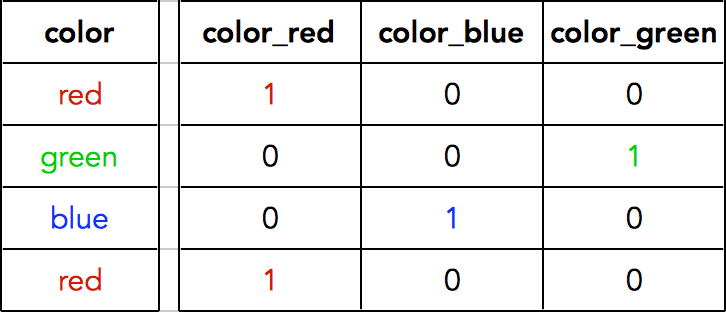
\includegraphics[width=0.6\textwidth]{Figures/one_hot_encoding}
	\caption{Ejemplo One hot encoding \\ Fuente:  \href{https://www.machinelearningplus.com/machine-learning/caret-package/attachment/one-hot-encoding/}{\textit{https://www.machinelearningplus.com/}}}
	\label{one}
\end{figure} 
En nuestra implementación fue necesario encontrar una representación para nuestras 10 clases de números. A continuación mostramos el código que nos permitió hallar esa representación.
\begin{lstlisting}[language=Python,caption=one hot encoding,captionpos=b,xleftmargin=.05\textwidth]
# importacion de libreria
from sklearn.preprocessing import OneHotEncoder
# vocabulario de clases definidas
vocabulary_words=np.array(['cero','uno','dos','tres',
'cuatro','cinco','seis','siete','ocho','nueve'])
# creacion del objeto OneHotEncoder
onehot_encoder = OneHotEncoder(handle_unknown='ignore',
categories='auto')
# entrenamiento del OneHotEncoder en base a las clases definidas
onehot_encoder.fit(X=vocabulary_words.reshape(-1,1))
\end{lstlisting}

\section{Modelo de la red neuronal}

En esta sección  veremos algunos modelos que fueron entrenados para la tarea de clasificación de audios de números estos serán probados con un solo tipo de redes RNN y en especial su derivado LSTM.
\subsection{RNN}
Definimos un red neuronal con una sola capa RNN y una capa densamente conectada.

\begin{lstlisting}[language=Python,caption=Modelo LSTM,captionpos=b,xleftmargin=.05\textwidth]
# establece la secuencia para empezar con el apilado de capas
model=tf.keras.Sequential()
# se apila una capa RNN simple 
model.add(tf.keras.layers.SimpleRNN(128, input_shape=(time_steps,n_inputs)))
# establece una capa densamente conectada
model.add(tf.layers.Dense(n_class, activation='softmax'))

\end{lstlisting}


\subsection{LSTM}
Para LSTM veremos modelo sin la aplicación de la capa Dropout y modelos con esta capa.


Nuestro modelo fue definido usando keras como muestra el código 5.3 

\begin{center}
\begin{lstlisting}[language=Python,caption=Modelo LSTM,captionpos=b,xleftmargin=.05\textwidth]
# usado para apilar las capas de la red
model=tf.keras.Sequential()
# apila una capa LSTM
model.add(tf.keras.layers.LSTM(n_units,
 input_shape=(time_steps,n_inputs)))
# apila un Dropout a nuestra red para evitar overfitting
model.add(tf.keras.layers.Dropout(0.5))
# establece una capa densamente conectada
model.add(tf.layers.Dense(n_class, activation='softmax'))


\end{lstlisting}
\end{center}



Para entrenamiento de nuestro modelos usaremos los parámetros mostrados en el código 5.4, categorical crossentropy será nuestra función de perdida y nuestro optimizador será Adam.s

\begin{lstlisting}[language=Python,caption=Parámetros para el entrenamiento del modelo,captionpos=b,xleftmargin=.05\textwidth]
# configura el entrenamiento del modelo
model.compile(loss='categorical_crossentropy',
optimizer='adam',metrics=['accuracy'])
\end{lstlisting}